%!TEX TS-program = xelatex
\documentclass[notes,12pt, aspectratio=169]{beamer}

\usepackage{amsmath,amsfonts,amssymb,amsthm,mathtools}  % пакеты для математики
%\usepackage{minted}

\usepackage[english, russian]{babel} % выбор языка для документа
\usepackage[utf8]{inputenc} % задание utf8 кодировки исходного tex файла
\usepackage[X2,T2A]{fontenc}        % кодировка

\usepackage{fontspec}         % пакет для подгрузки шрифтов
\setmainfont{Georgia}  % задаёт основной шрифт документа

% why do we need \newfontfamily:
% http://tex.stackexchange.com/questions/91507/
\newfontfamily{\cyrillicfonttt}{Georgia}
\newfontfamily{\cyrillicfont}{Georgia}
\newfontfamily{\cyrillicfontsf}{Georgia}

\usepackage{unicode-math}     % пакет для установки математического шрифта
% \setmathfont{Neo Euler} % шрифт для математики

\usepackage{polyglossia}      % Пакет, который позволяет подгружать русские буквы
\setdefaultlanguage{russian}  % Основной язык документа
\setotherlanguage{english}    % Второстепенный язык документа

% Шрифт для кода
\setmonofont[Scale=0.85]{Georgia}
\usepackage{verbments}

\usepackage{pgfpages}
% These slides also contain speaker notes. You can print just the slides,
% just the notes, or both, depending on the setting below. Comment out the want
% you want.
%\setbeameroption{hide notes} % Only slide
%\setbeameroption{show only notes} % Only notes
%\setbeameroption{show notes on second screen=right} % Both

\usepackage{array}

\usepackage{tikz}
\usepackage{verbatim}
\setbeamertemplate{note page}{\pagecolor{yellow!5}\insertnote}
\usetikzlibrary{positioning}
\usetikzlibrary{snakes}
\usetikzlibrary{calc}
\usetikzlibrary{arrows}
\usetikzlibrary{decorations.markings}
\usetikzlibrary{shapes.misc}
\usetikzlibrary{matrix,shapes,arrows,fit,tikzmark}

\usepackage{hyperref}
\usepackage{lipsum}
\usepackage{multimedia}
\usepackage{multirow}
\usepackage{dcolumn}
\usepackage{bbm}
\newcolumntype{d}[0]{D{.}{.}{5}}

\usepackage{changepage}
\usepackage{appendixnumberbeamer}
\newcommand{\beginbackup}{
	\newcounter{framenumbervorappendix}
	\setcounter{framenumbervorappendix}{\value{framenumber}}
	\setbeamertemplate{footline}
	{
		\leavevmode%
		\hline
		box{%
			\begin{beamercolorbox}[wd=\paperwidth,ht=2.25ex,dp=1ex,right]{footlinecolor}%
				%         \insertframenumber  \hspace*{2ex} 
		\end{beamercolorbox}}%
		\vskip0pt%
	}
}
\newcommand{\backupend}{
	\addtocounter{framenumbervorappendix}{-\value{framenumber}}
	\addtocounter{framenumber}{\value{framenumbervorappendix}} 
}

% для имитации питоновского синтаксиса 
\newcommand{\pgr}[1]{{\color{green} \textbf{#1}}}


%%%%%%%%%% Работа с картинками %%%%%%%%%
\usepackage{graphicx}                  % Для вставки рисунков
\usepackage{graphics}
\graphicspath{{images/}}    % можно указать папки с картинками
\usepackage{wrapfig}                   % Обтекание рисунков и таблиц текстом

\usepackage[space]{grffile}
\usepackage{booktabs}

% These are my colors -- there are many like them, but these ones are mine.
\definecolor{blue}{RGB}{0,114,178}
\definecolor{red}{RGB}{213,94,0}
\definecolor{yellow}{RGB}{240,228,66}
\definecolor{green}{RGB}{0,128, 0}

\hypersetup{
	colorlinks=false,
	linkbordercolor = {white},
	linkcolor = {blue}
}


%% I use a beige off white for my background
\definecolor{MyBackground}{RGB}{255,253,218}

%% Uncomment this if you want to change the background color to something else
%\setbeamercolor{background canvas}{bg=MyBackground}

%% Change the bg color to adjust your transition slide background color!
\newenvironment{transitionframe}{
	\setbeamercolor{background canvas}{bg=yellow}
	\begin{frame}}{
\end{frame}
}

\setbeamercolor{frametitle}{fg=blue}
\setbeamercolor{title}{fg=black}
\setbeamertemplate{footline}[frame number]
\setbeamertemplate{navigation symbols}{} 
\setbeamertemplate{itemize items}{-}
\setbeamercolor{itemize item}{fg=blue}
\setbeamercolor{itemize subitem}{fg=blue}
\setbeamercolor{enumerate item}{fg=blue}
\setbeamercolor{enumerate subitem}{fg=blue}
\setbeamercolor{button}{bg=MyBackground,fg=blue,}
\usepackage{hyperref}
\usepackage{graphicx}

% If you like road maps, rather than having clutter at the top, have a roadmap show up at the end of each section 
% (and after your introduction)
% Uncomment this is if you want the roadmap!
% \AtBeginSection[]
% {
%    \begin{frame}
%        \frametitle{Roadmap of Talk}
%        \tableofcontents[currentsection]
%    \end{frame}
% }
\setbeamercolor{section in toc}{fg=blue}
\setbeamercolor{subsection in toc}{fg=red}
\setbeamersize{text margin left=1em,text margin right=1em} 

% списки, которые растягиваются на всю величину слайда 
\newenvironment{wideitemize}{\itemize\addtolength{\itemsep}{10pt}}{\enditemize}



\title[]{\textcolor{blue}{Глубокое обучение и вообще}}
\author{Ульянкин Филипп и Соловей Влад}
\date{\today}


\begin{document}

%%% TIKZ STUFF
\tikzset{   
        every picture/.style={remember picture,baseline},
        every node/.style={anchor=base,align=center,outer sep=1.5pt},
        every path/.style={thick},
        }
\newcommand\marktopleft[1]{%
    \tikz[overlay,remember picture] 
        \node (marker-#1-a) at (-.3em,.3em) {};%
}
\newcommand\markbottomright[2]{%
    \tikz[overlay,remember picture] 
        \node (marker-#1-b) at (0em,0em) {};%
}
\tikzstyle{every picture}+=[remember picture] 
\tikzstyle{mybox} =[draw=black, very thick, rectangle, inner sep=10pt, inner ysep=20pt]
\tikzstyle{fancytitle} =[draw=black,fill=red, text=white]
%%%% END TIKZ STUFF

% Title Slide
\begin{frame}
\maketitle
\centering \textbf{\color{blue} Посиделка 13:} Быстрое введение в  SOTA 
\end{frame}


\begin{frame}{Agenda} 
\begin{wideitemize}
	\item  Быстрая история
	\item  seq2seq
	\item  Attention
	\item  Self-attention
	\item  BERT
	\item  ELMO
	\item  Сломанный мозг.....
\end{wideitemize}
\end{frame}


\begin{transitionframe}
	\begin{center}
		\Huge  Быстренькая история взятая из старых лекций
	\end{center}
\end{transitionframe}

\begin{transitionframe}
	\begin{center}
		\Huge  задача seq2seq
	\end{center}
\end{transitionframe}




\begin{frame}{спойлер}
\centering После этой лекции могут возникнуть огромное количество вопросов - но в современных архитектурах слишком много инженерных хаков, которые лучше осозновать постепенно сами.

Я буду оставлять некоторые ключевые слова того, чтобы вы могли сами залезть поглубже, если такое погружение потребуется.
\end{frame}


\begin{frame}
\centering Задача seq2seq  - задача, когда мы хотим предсказать по одной последовательности другую
Самая стандартная подобная задача - машинный перевод. Нейронные сети ворвались в эту сферу человеческого прогресса в 2014 году
\end{frame}

\begin{frame}{Метрика}

Модели в машинном переводе сравнивают по BLEU score - если в кратце, то эта метрика сравнения полученного машиной перевода и человеческого, насколько мы вообще бьемся. Из проблем данной метрики - если машина перевела правильно, но альтернативно, то BLEU будет низкий....
\end{frame}

\begin{frame}
	\begin{figure}
		\centering
		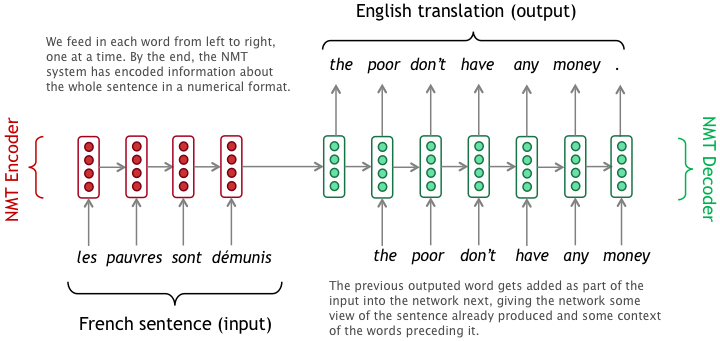
\includegraphics[width=1\linewidth]{images/seq2seq}
		\label{fig:seq2seq}
	\end{figure}
\end{frame}

\begin{frame}{Greedy decoding}

При декодировании может быть следующие проблемы - мы декодируем какое-то конкретное слово.
Но что делать если это слово некоректное?
\end{frame}

\begin{frame}{Greedy decoding/beam search}

Самый простой подход - селектить несколько наиболее вероятных слов, а не одно. Мы получим множество предложений, а потом по какой-то эвристике выбирать лучшее из них. Подход хорош всем, кроме скорости.

Ему есть альтернатива - называется beam-search.
\end{frame}

\begin{frame}

Какие проблемы мы видим в таком подходе (спойлер, из коробки он не полетел)?
\end{frame}


\begin{transitionframe}
	\begin{center}
		\Huge  Attention!
	\end{center}
\end{transitionframe}

\begin{frame}{Attention}
А вот бы использовать не один вектор, а все. Информация то течет и кодируется во всех векторах.....

И да - это классная и разумная идея. Нам на встречу приходит концепция внимания.

\end{frame}


\begin{frame}{Attention}
		\begin{figure}
		\centering
		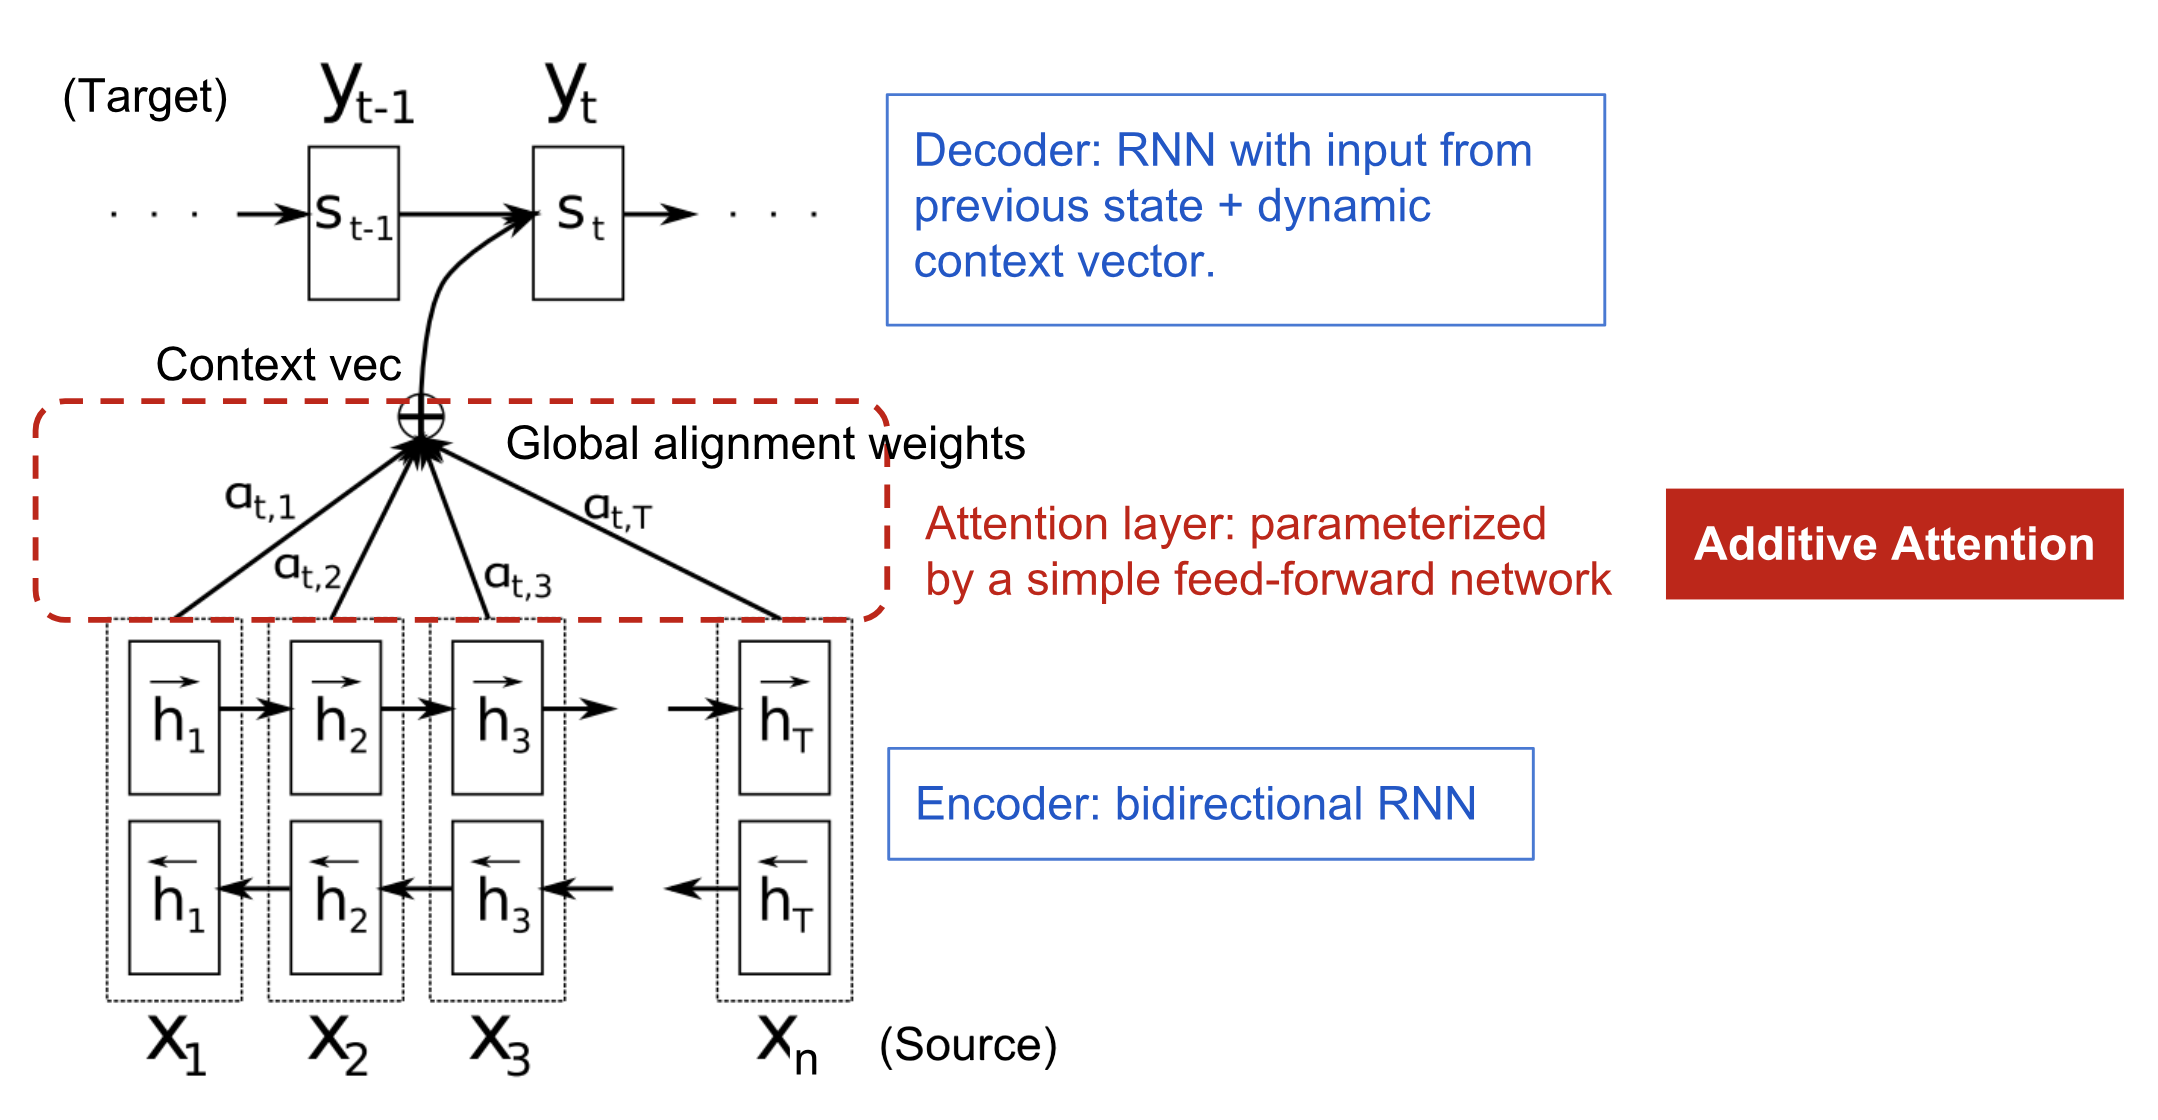
\includegraphics[width=0.8\linewidth]{images/encoder-decoder-attention}
		\label{fig:seq2seq}
	\end{figure}

	
\end{frame}

\begin{frame}{Attention}

	\begin{figure}
	\centering
	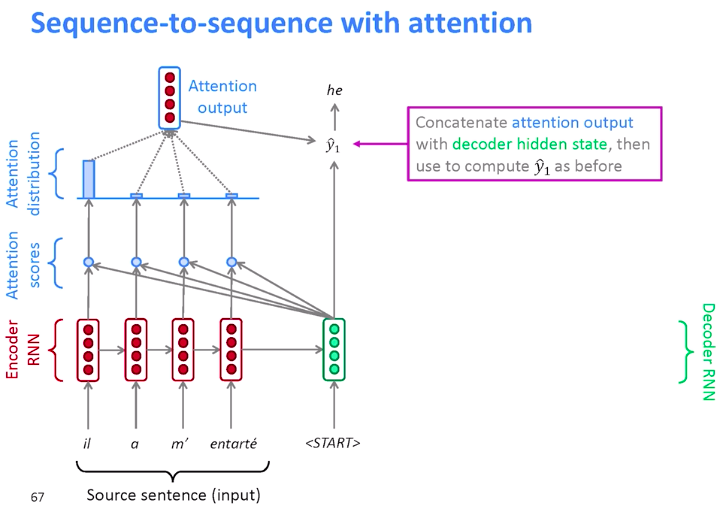
\includegraphics[width=0.6\linewidth]{images/attention_1}
	\label{fig:seq2seq}
\end{figure}
\href{https://mc.ai/attention-in-deep-learning/}{\textbf{ссылочка на оригинал}}
\end{frame}

\begin{frame}{Attention}

\begin{figure}
	\centering
	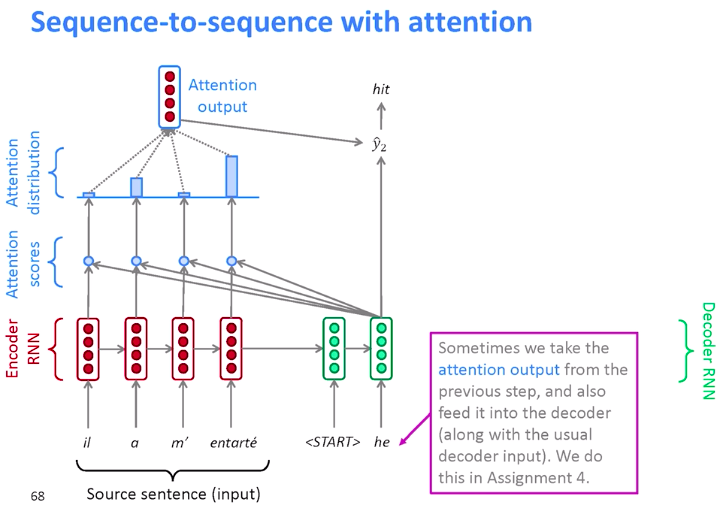
\includegraphics[width=0.7\linewidth]{images/attention_2}
	\label{fig:seq2seq}
\end{figure}
\end{frame}

\begin{frame}{Attention}

\begin{figure}
	\centering
	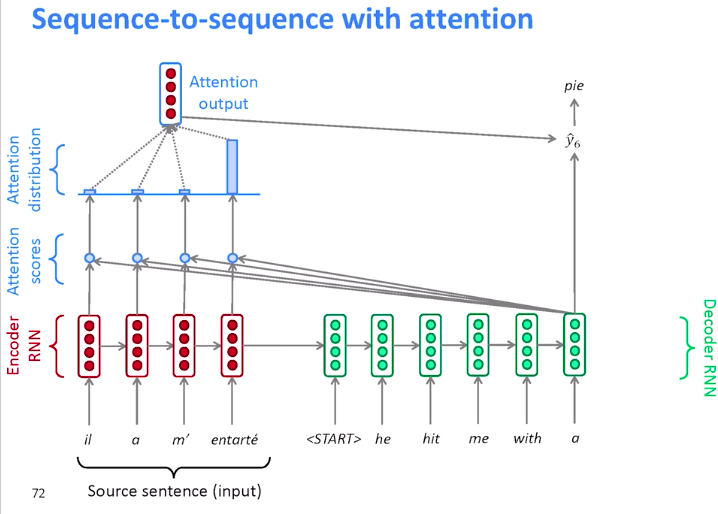
\includegraphics[width=0.7\linewidth]{images/attention_3}
	\label{fig:seq2seq}
\end{figure}
\end{frame}

\begin{frame}{Attention}

\begin{figure}
	\centering
	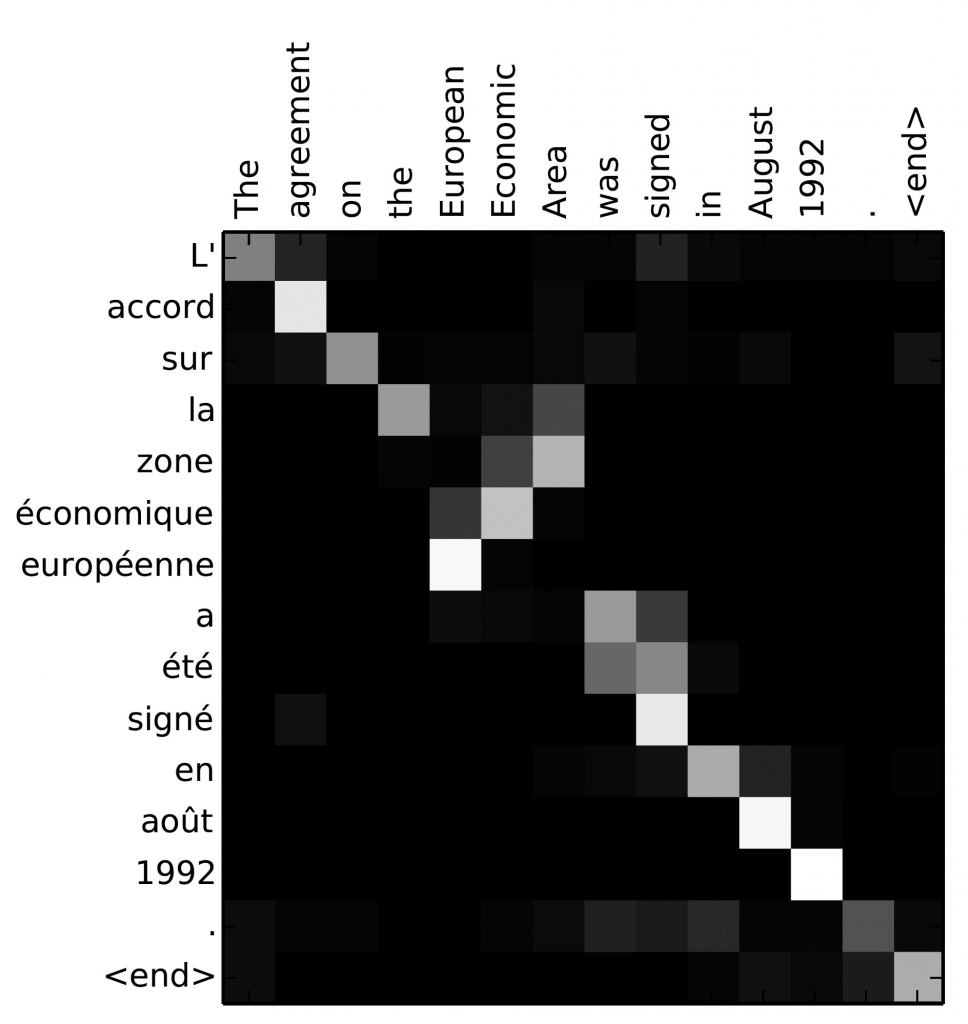
\includegraphics[width=0.5\linewidth]{images/undestend_attention}
	\label{fig:seq2seq}
\end{figure}
\end{frame}


\begin{frame}{Attention}

\begin{figure}
	\centering
	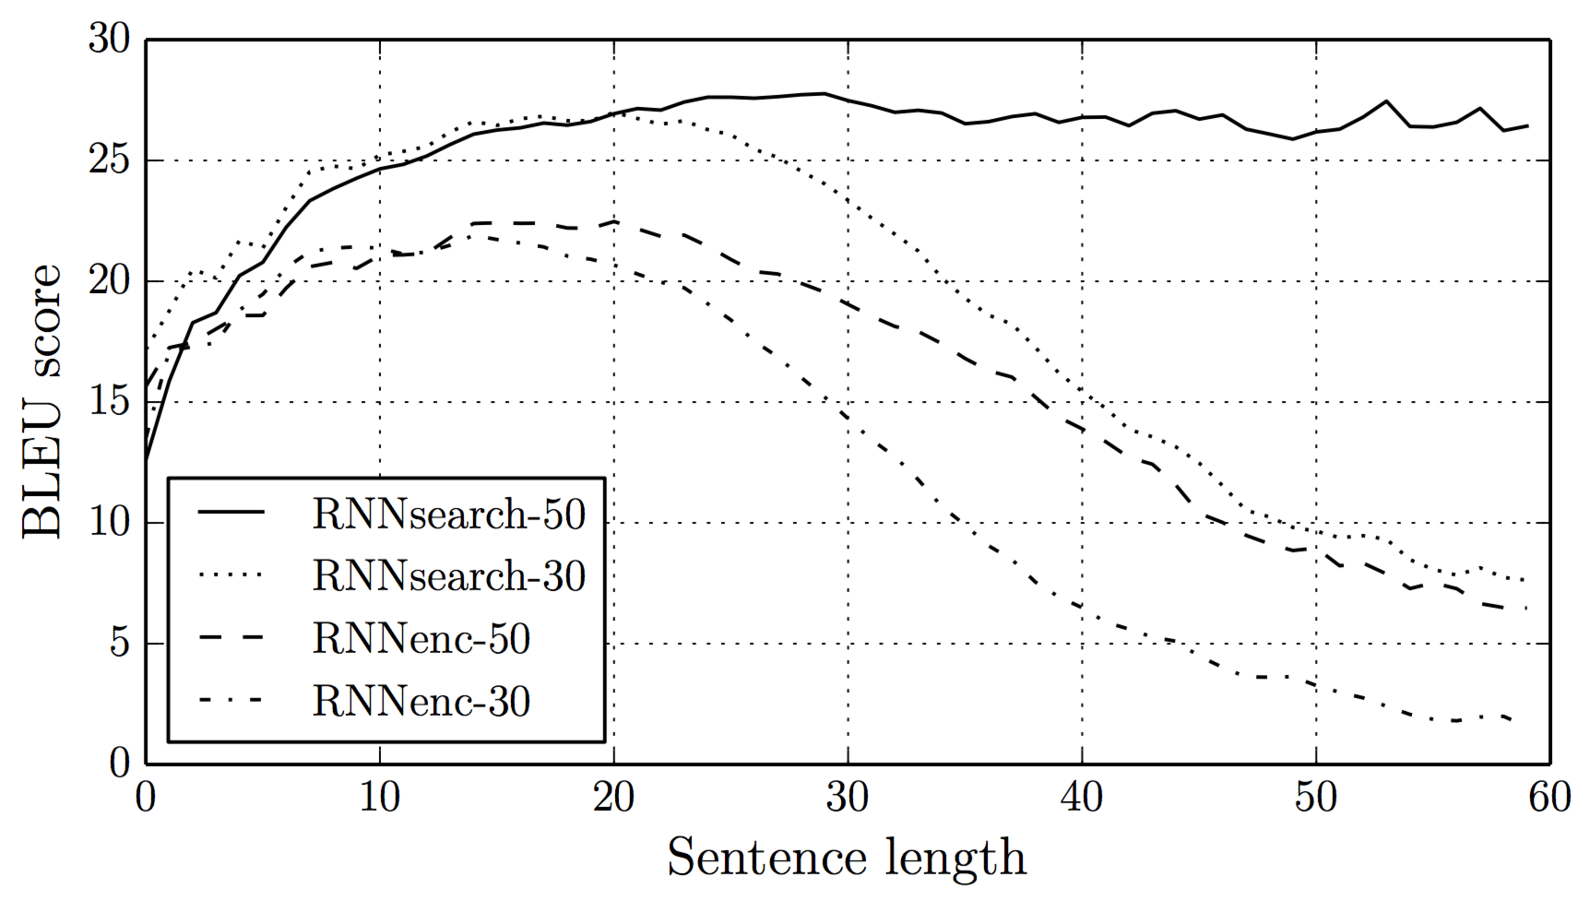
\includegraphics[width=1\linewidth]{images/bahdanau_attn}
	\label{fig:seq2seq}
\end{figure}
\end{frame}


\begin{frame}{Attention}

Идейно - внимание просто выбирает то из эмбедингов, которое действительно нужно для декодирования.
Это просто матричное произведение(а можно взвешивать и без весов) и softmax. У нас все остается дифферинцируемым - берем градиентны, накапливаем инфу в весах сетки. 
\end{frame}

\begin{frame}{google}
\begin{figure}
	\centering
	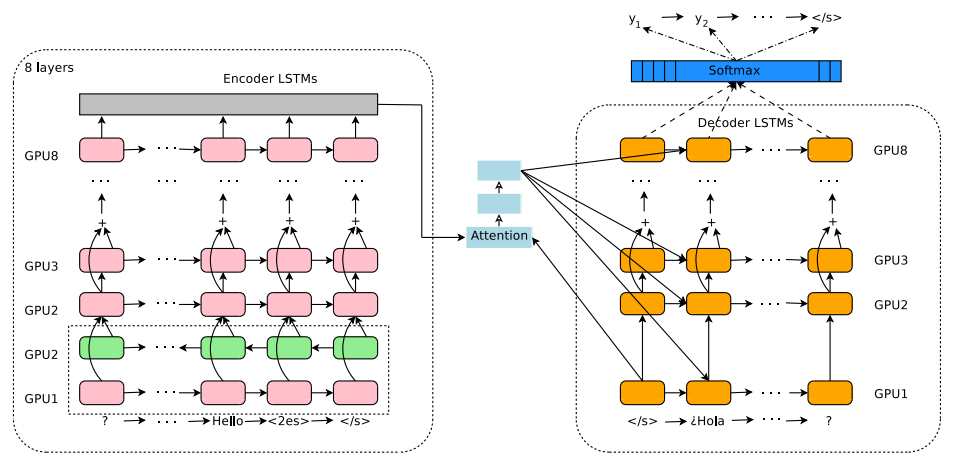
\includegraphics[width=1\linewidth]{images/google_neural_first}
	\label{fig:seq2seq}
\end{figure}
\end{frame}


\begin{frame}{google}
В целом глобальное решение было найдено, осталось закидать проблему железом.

Выводы:
\begin{enumerate}
	\item 8 слоев LSTM (8 Карл!)
	\item в attention 2 слоя dense. 
	\item Собираем слова из морфем - пытаемся победить out-of-vacabular.
	\item Модель стала иногда сексистом и фашистом - требуются слишком большие дата сеты, чтобы учить эту большую прелесть.
\end{enumerate}
\end{frame}

\begin{transitionframe}
	\begin{center}
		\Huge  Attention is all you need!
	\end{center}
\end{transitionframe}

\begin{frame}{attention is all you need}
Развитие идеи внимания. Статья вышла в 2017 году и стала мамой всех текущих SOTA моделей.
А зачем нам вообще что-то, кроме внимания?
Давайте напихаем в энкодер и декодер как можно больше внимания и будем такой штукой его учить.
\end{frame}


\begin{frame}{attention is all you need}
\begin{figure}
	\centering
	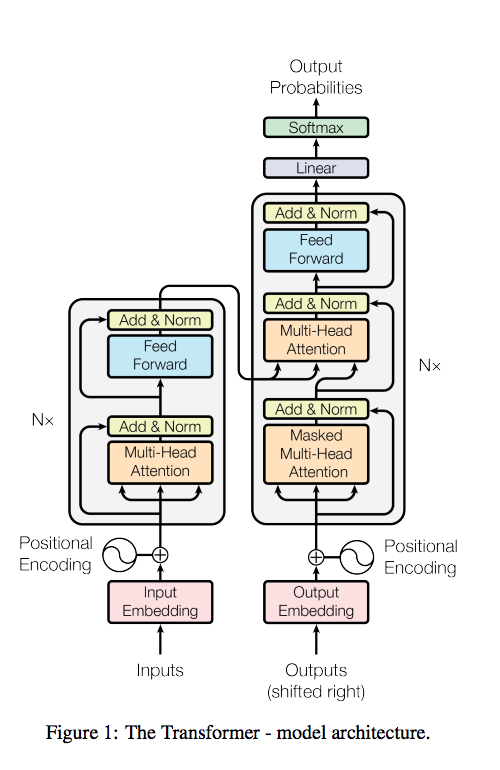
\includegraphics[width=0.37\linewidth]{images/all_attention}
	\label{fig:seq2seq}
\end{figure}
\end{frame}


\begin{frame}{Encoder}
\begin{figure}
	\centering
	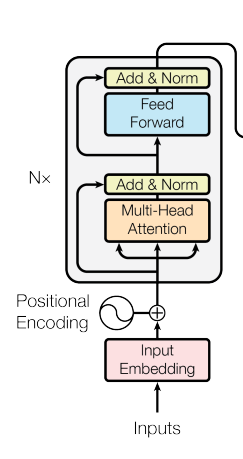
\includegraphics[width=0.28\linewidth]{images/encoder}
	\label{fig:seq2seq}
\end{figure}
\end{frame}


\begin{frame}{Что мы хотим?}
Есть предложение:
”The animal didn't cross the street because it was too tired”
\begin{figure}
	\centering
	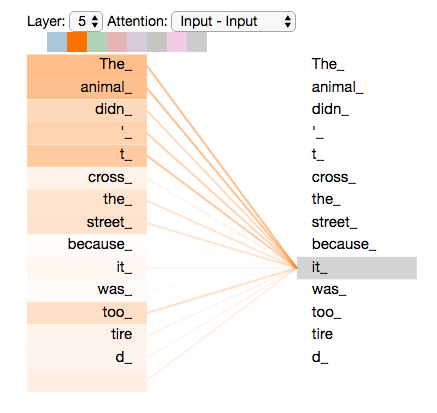
\includegraphics[width=0.37\linewidth]{images/transformer_self-attention_visualization}
	\label{fig:seq2seq}
\end{figure}
\end{frame}

\begin{frame}{Абстракции!}
\begin{figure}
	\centering
	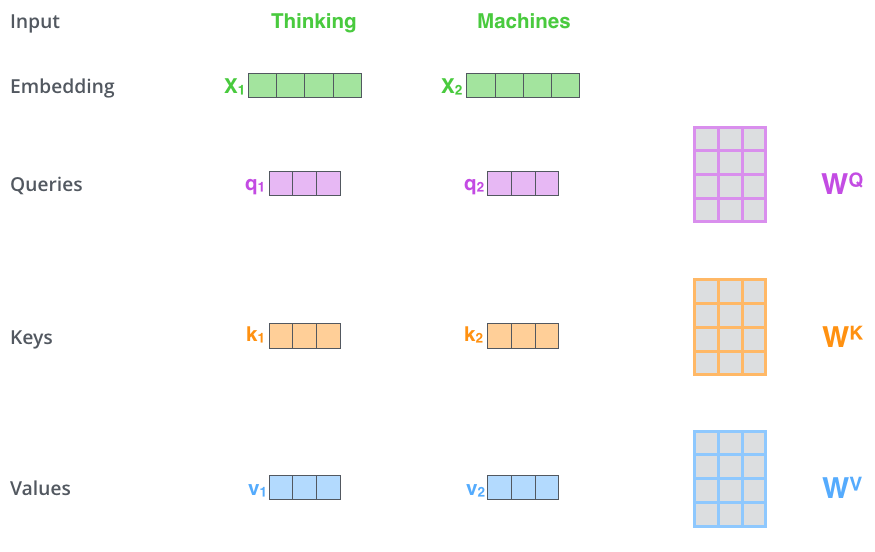
\includegraphics[width=0.8\linewidth]{images/transformer_self_attention_vectors}
	\label{fig:seq2seq}
\end{figure}
\end{frame}


\begin{frame}
А теперь тоже самое, но словами:
\begin{enumerate}
	\item Query,key - ищем связи между словами. Ходим по всем со всеми смотрим насколько они связаны. Query - мое текущее слово, key - мое слово с которым я сравниваю себя.
	\item Value - то, что мы знаем об этом слове
\end{enumerate}
\end{frame}

\begin{frame}{Шаг 2}
\begin{figure}
	\centering
	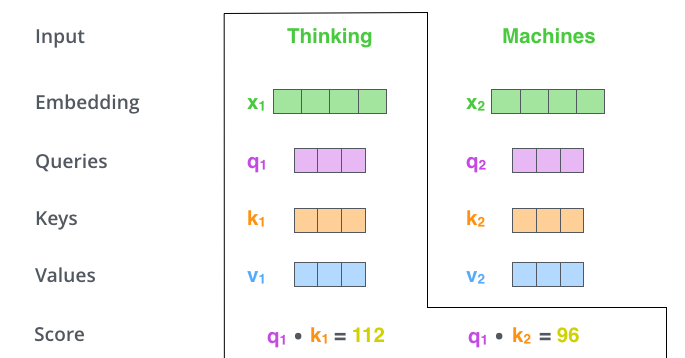
\includegraphics[width=0.8\linewidth]{images/step_2}
	\label{fig:seq2seq}
\end{figure}
\end{frame}

\begin{frame}{Шаг 3}
\begin{figure}
	\centering
	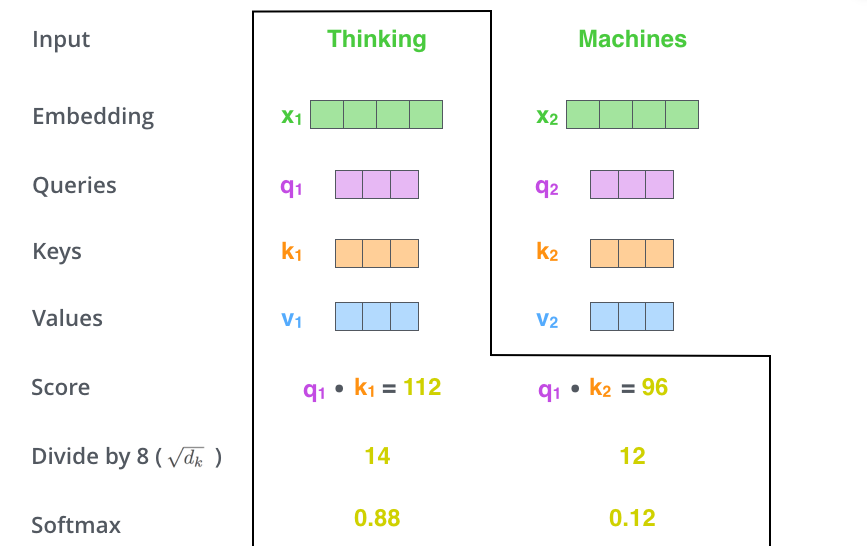
\includegraphics[width=0.8\linewidth]{images/step_3}
	\label{fig:seq2seq}
\end{figure}
\end{frame}

\begin{frame}{Шаг 4}
\begin{figure}
	\centering
	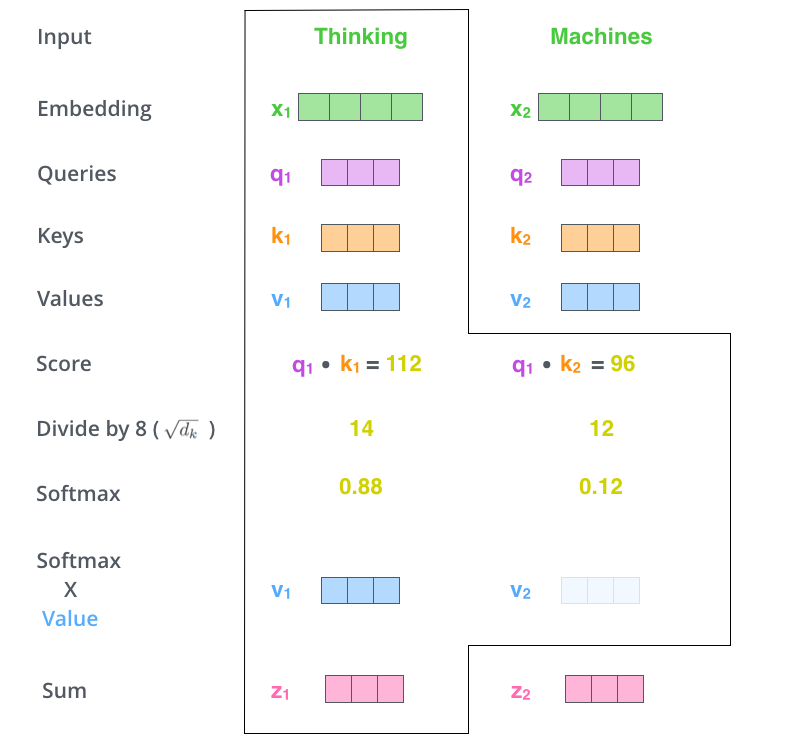
\includegraphics[width=0.5\linewidth]{images/step_4}
	\label{fig:seq2seq}
\end{figure}
\end{frame}

\begin{frame}{Шаг 5}
\begin{figure}
	\centering
	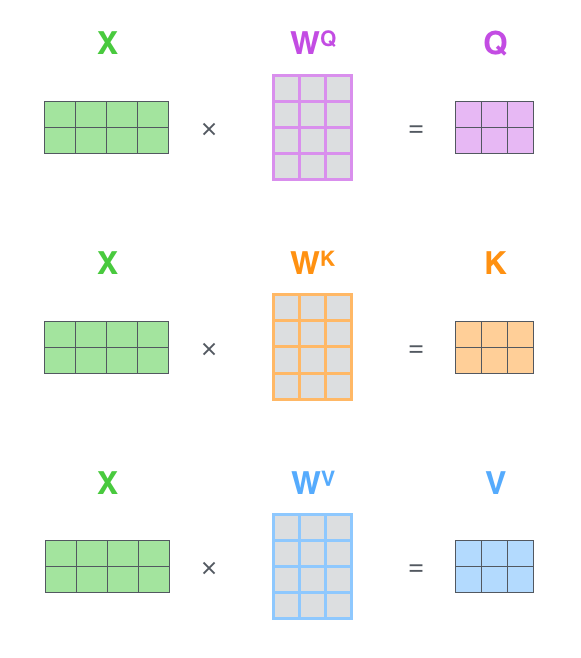
\includegraphics[width=0.4\linewidth]{images/step_5}
	\label{fig:seq2seq}
\end{figure}
\end{frame}

\begin{frame}{multi head attention}
\begin{figure}
	\centering
	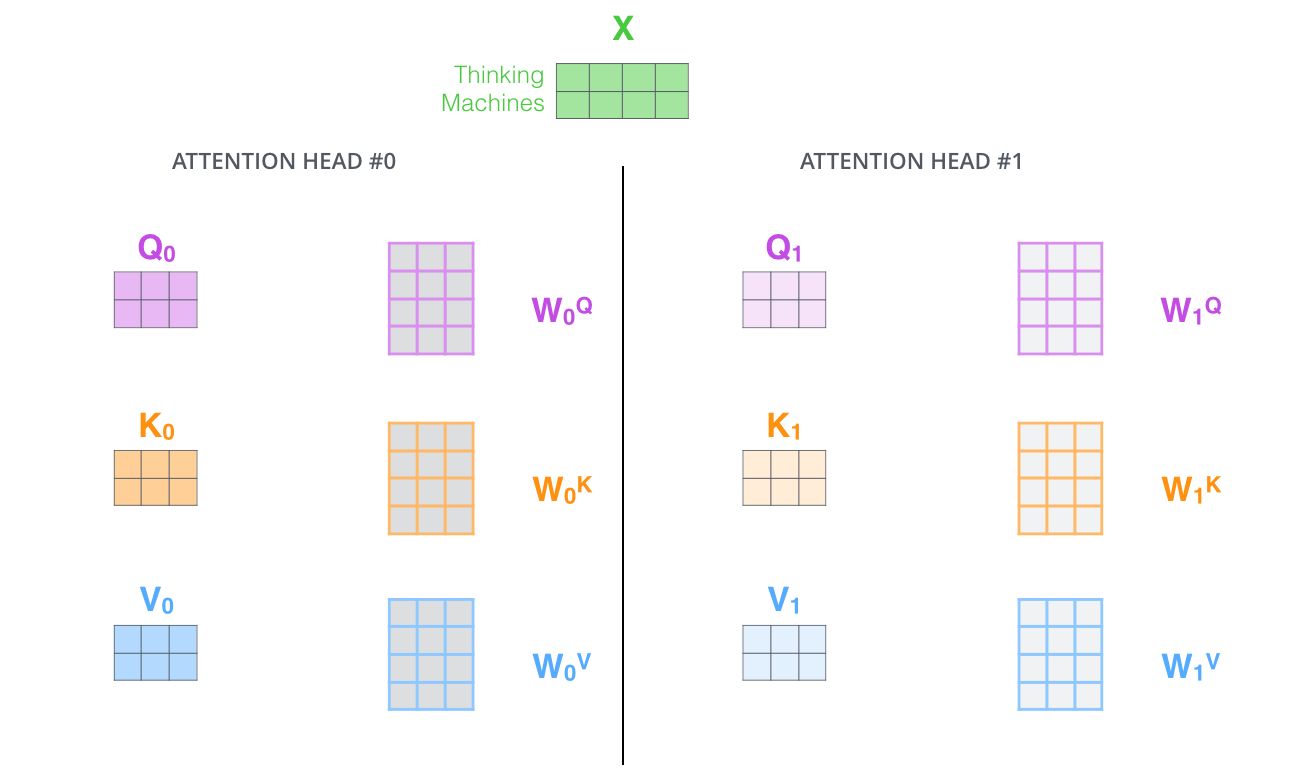
\includegraphics[width=0.8\linewidth]{images/multi_heads}
	\label{fig:seq2seq}
\end{figure}
\end{frame}

\begin{frame}{Соединяем!}
\begin{figure}
	\centering
	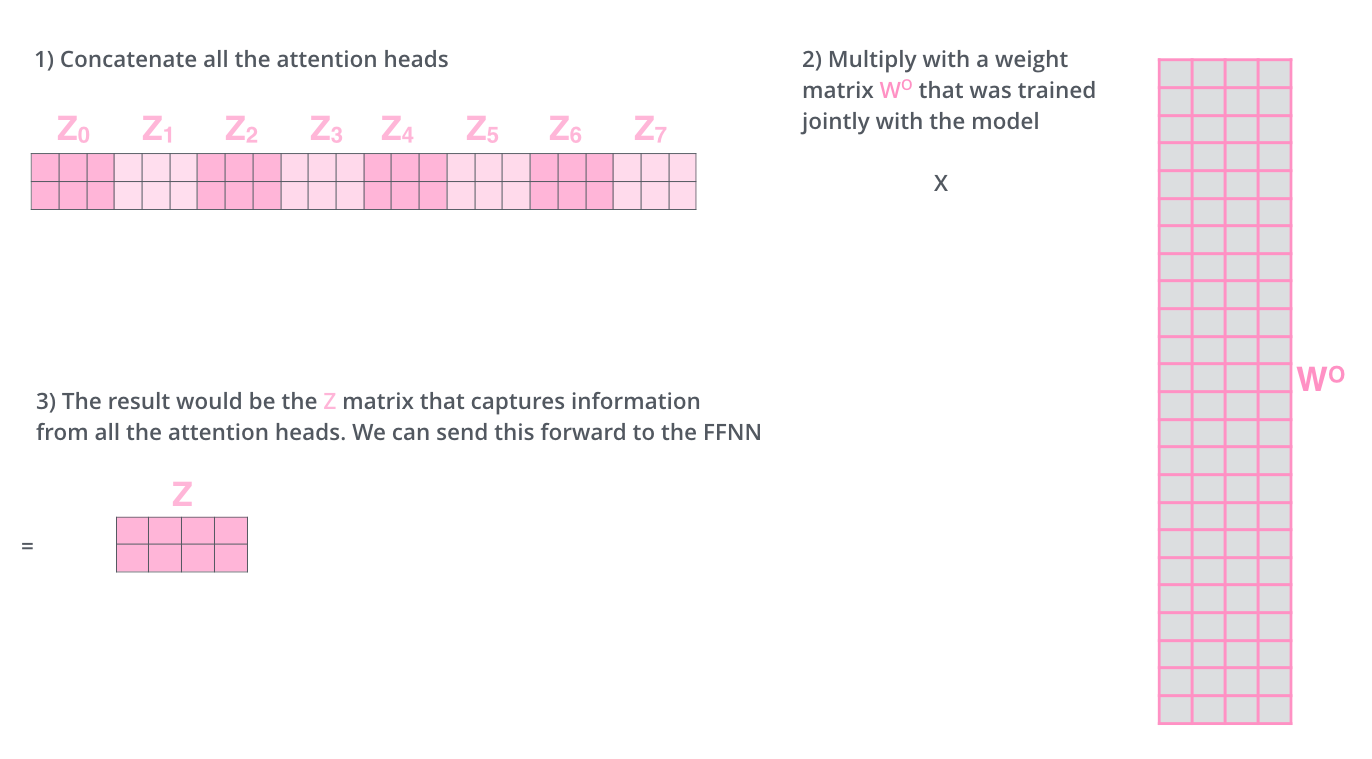
\includegraphics[width=0.8\linewidth]{images/transformer_attention_heads_weight_matrix_o}
	\label{fig:seq2seq}
\end{figure}
\end{frame}

\begin{frame}{Итого}
\begin{figure}
	\centering
	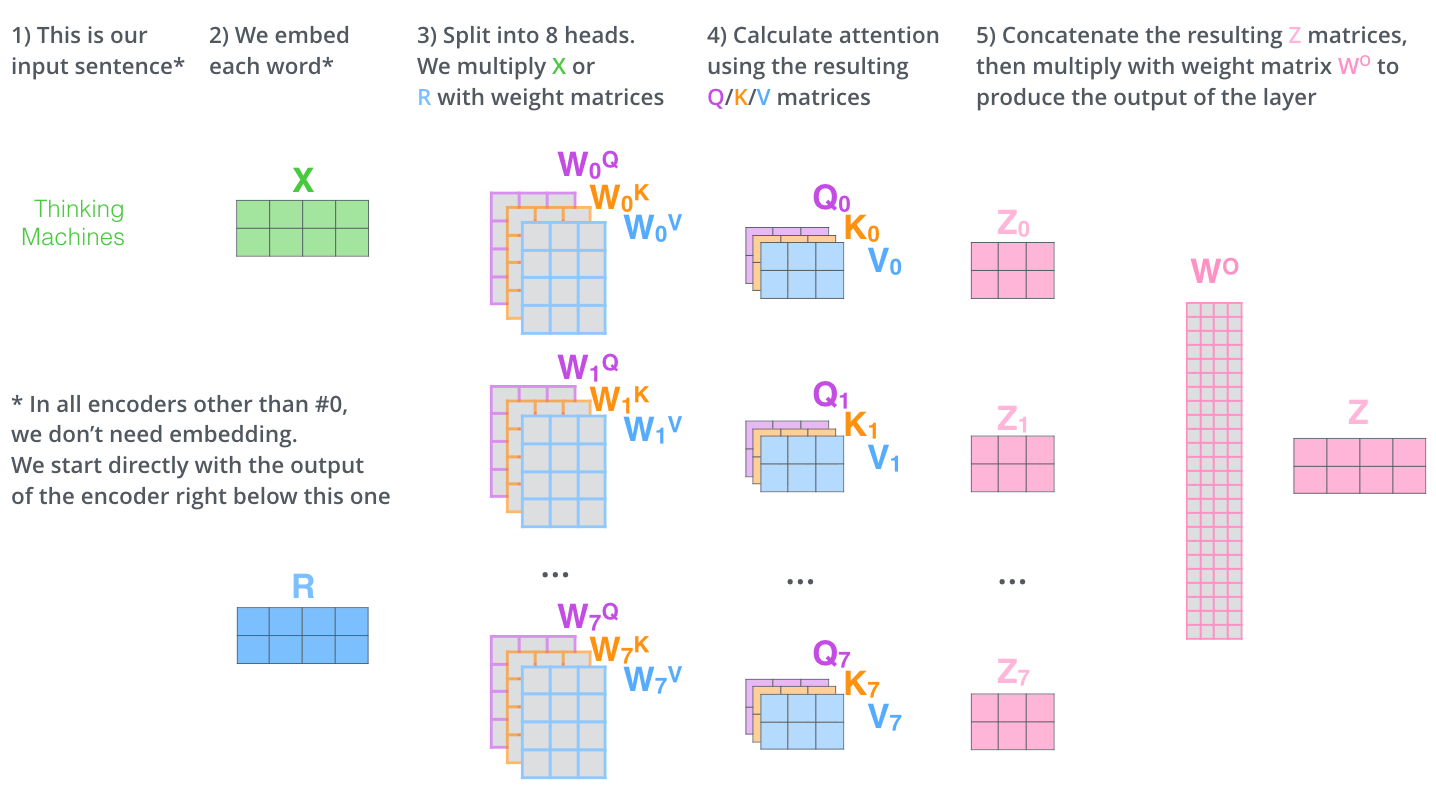
\includegraphics[width=0.8\linewidth]{images/final_attention}
	\label{fig:seq2seq}
\end{figure}
\end{frame}

\begin{frame}{Итого}
\begin{figure}
	\centering
	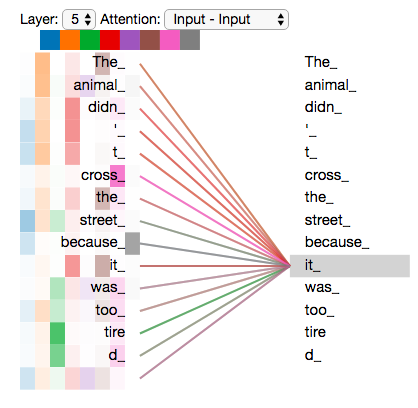
\includegraphics[width=0.5\linewidth]{images/transformer_self-attention_visualization_3}
	\label{fig:seq2seq}
\end{figure}
\end{frame}


\begin{frame}{Итого}
Выходом всего этого дела будут вектора key и value, которые позволят декодеру смотреть на нужные нам кусочки.
И бежим смотреть гифки декодера!

Объяснение взято отсюда \href{http://jalammar.github.io/illustrated-transformer/}{\textbf{английский оригинал}} и отсюда \href{https://www.youtube.com/watch?v=Bg8Y5q1OiP0&list=PL4_hYwCyhAvZeq93ssEUaR47xhvs7IhJM&index=4}{\textbf{лекции мфти}}
\end{frame}

\begin{frame}{Итого}
\begin{enumerate}
	\item У нас нет никаких слоев, кроме dense
	\item Учится очень классно, находит множество взаимосвязей
	\item позицион энкодинг позволяет учитывать позицию в тексте 
\end{enumerate}


\end{frame}

\begin{frame}
\begin{figure}
	\centering
	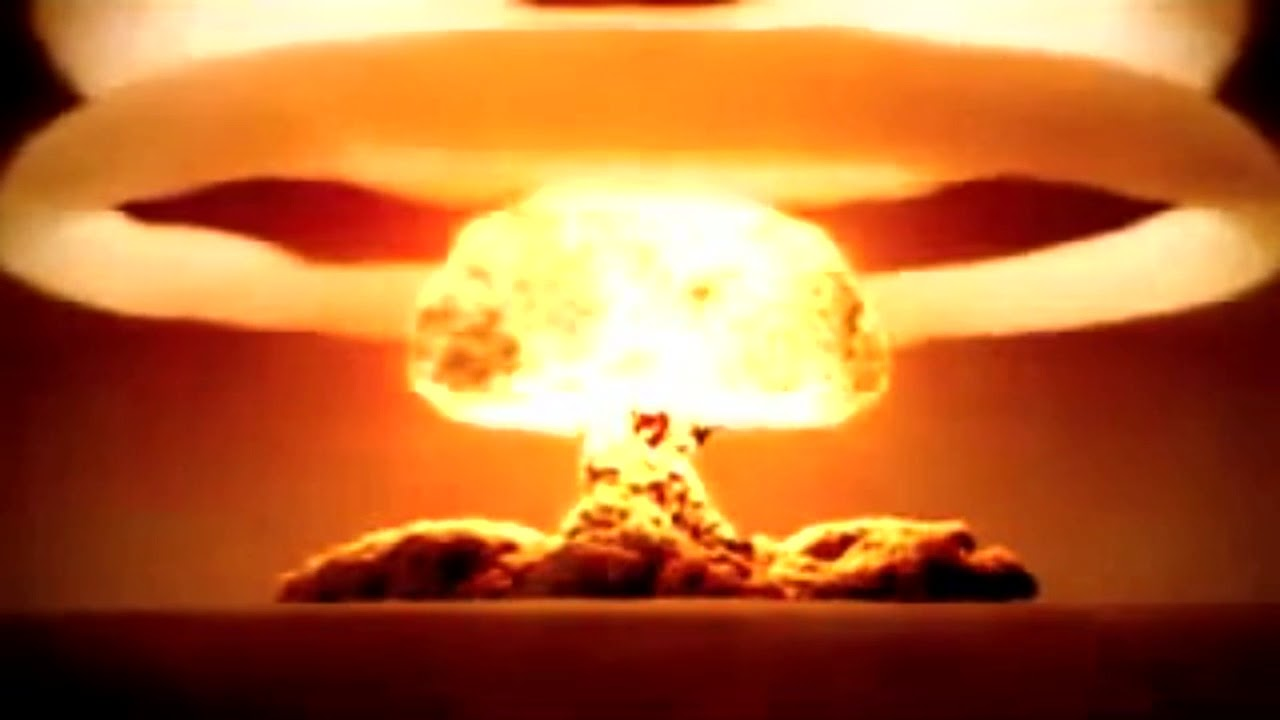
\includegraphics[width=0.8\linewidth]{images/maxresdefault}
	\label{fig:seq2seq}
\end{figure}
\textbf{И понеслась!!!} (развитие дальше - инженерные хаки и закидывание железом)
\end{frame}

\begin{transitionframe}
	\begin{center}
		\Huge  SOTA (ну или история соты)
	\end{center}
\end{transitionframe}

\begin{frame}
Крутой обзорчик с техническими деталями - живут в тех же лекция физтеха. При желании можно вкурить. И да, в целом курс достаточно крутой - и крут он тем, что считается, что слушатель не лаптем щи хлебает, а считает градиент на лету, но пока не придумал зачем.

\href{https://www.youtube.com/watch?v=iClc5dll8YU&list=PL4_hYwCyhAvZeq93ssEUaR47xhvs7IhJM&index=5}{\textbf{Обзор}}
\end{frame}

\begin{frame}{BERT}
Шел 2018 год и гугл сказал - наши комьютеры самые мощные, а данные самые большие!

BERT - Bidirectional Encoder Representations from Transformers

Почему круто - придумали как предобучать без учителя (да, вот оно, вот он наш космос). И потом переиспользовать веса!
\end{frame}


\begin{frame}{BERT}

\begin{figure}
	\centering
	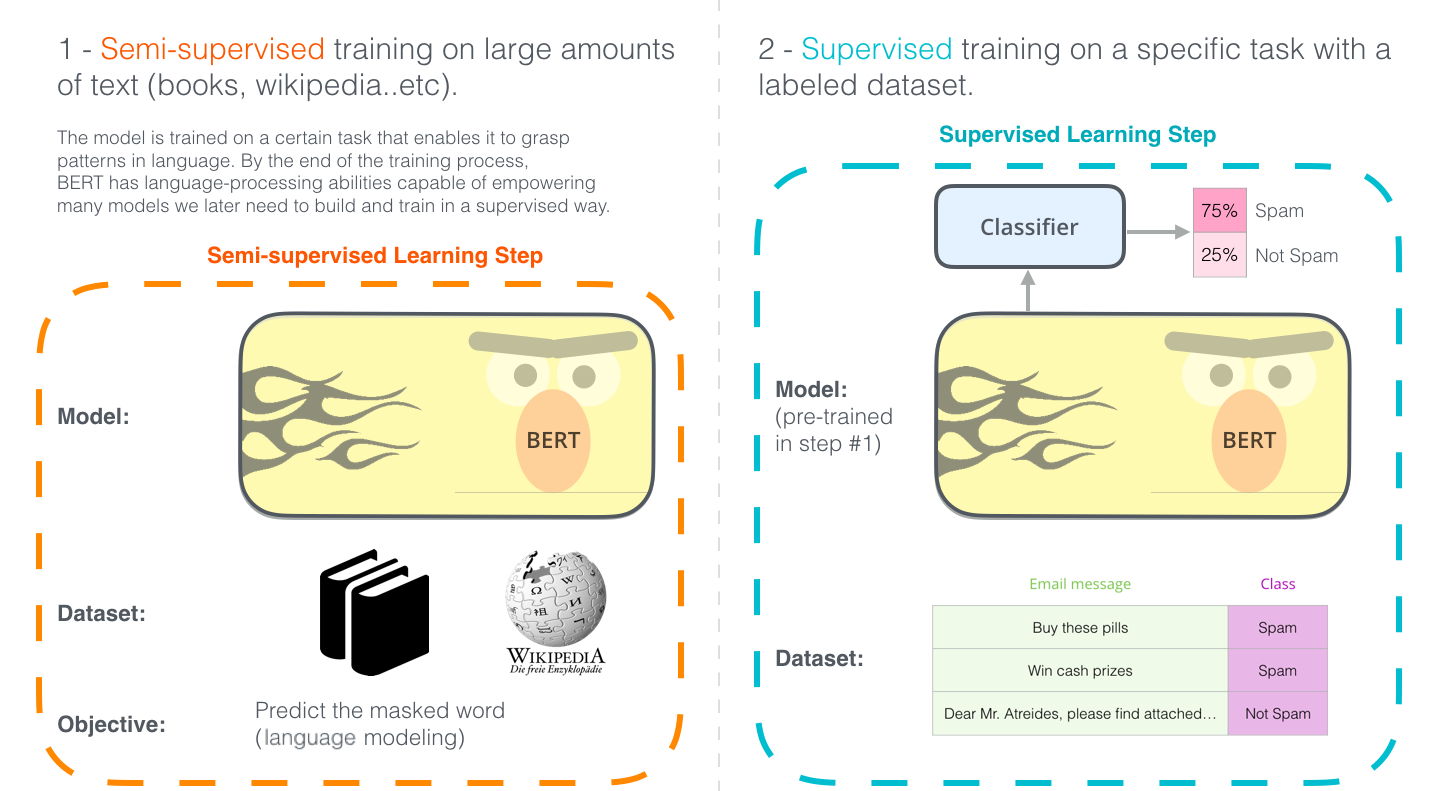
\includegraphics[width=0.9\linewidth]{images/BERT_stud}
	\label{fig:seq2seq}
\end{figure}

\end{frame}


\begin{frame}{BERT}
\begin{figure}
	\centering
	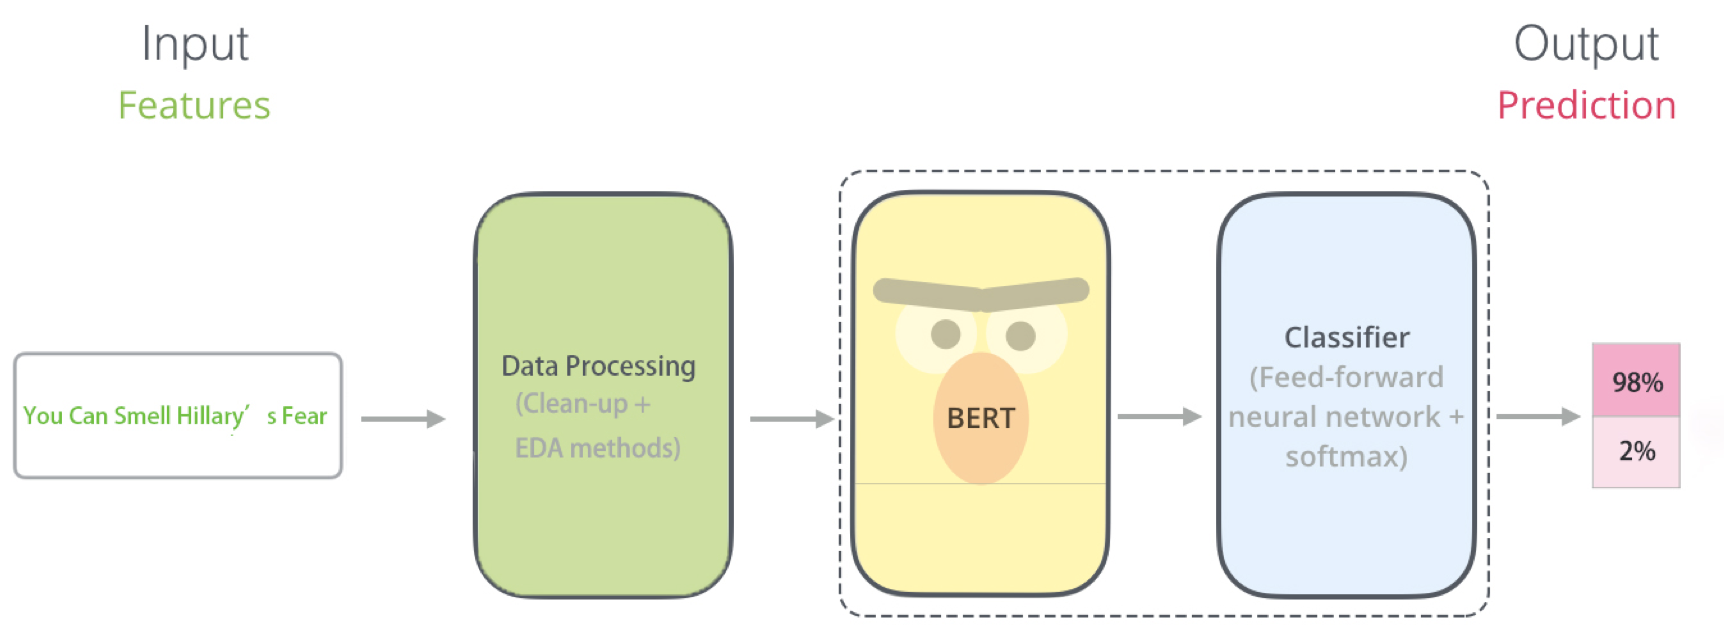
\includegraphics[width=0.9\linewidth]{images/use_bert}
	\label{fig:seq2seq}
\end{figure}
\end{frame}

\begin{frame}{Лежащие внутри идеи и почему он популярный}
\begin{enumerate}
	\item Предобучаем по двум задачам - берем корпус текстов и маскируем часть предложений, заставляем учить и предсказывать маску.
	\item И вторая идея - предсказываем следующее слово в предложении
	\item Он из коробки знает язык, ему 1-2 эпохи надо подсказать, что с этим знанием делать
	\item В готовых либах лежат много готовых под задачи бертов - классификация, вопросно - ответные системы и тому подобное.
	\item Опять же - подаем слова кусочками, чтобы как-то решать проблему oov.
\end{enumerate}
Все мы всех победили - нам не нужно размечать данные для обучения, мы счастливы!

\href{http://jalammar.github.io/illustrated-bert/}{\textbf{Обзорчик на забугорном}}
\end{frame}



\begin{frame}{предобучение}
\begin{figure}
	\centering
	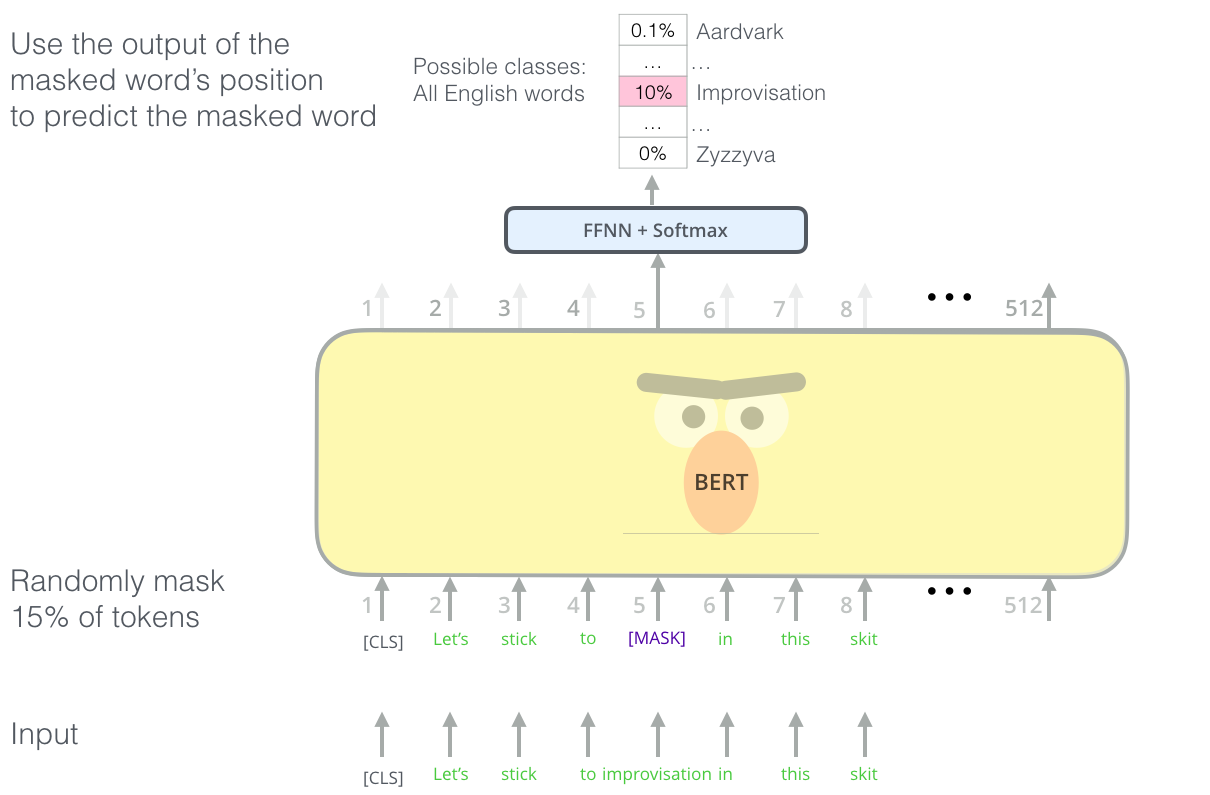
\includegraphics[width=0.75\linewidth]{images/pre_train_bert}
\end{figure}
\end{frame}

\begin{frame}{Как используем?}
\begin{figure}
	\centering
	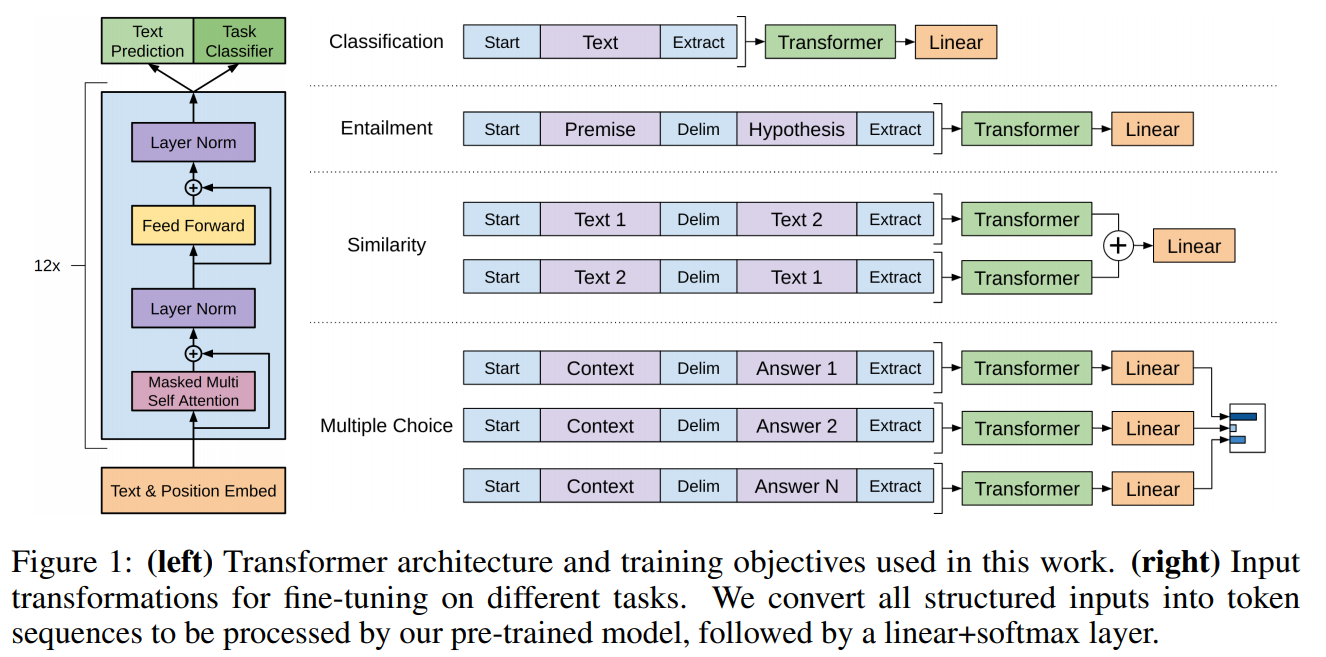
\includegraphics[width=0.9\linewidth]{images/use_models}
	\label{fig:seq2seq}
\end{figure}
\end{frame}

\begin{frame}{Почему заработало?}
\begin{figure}
	\centering
	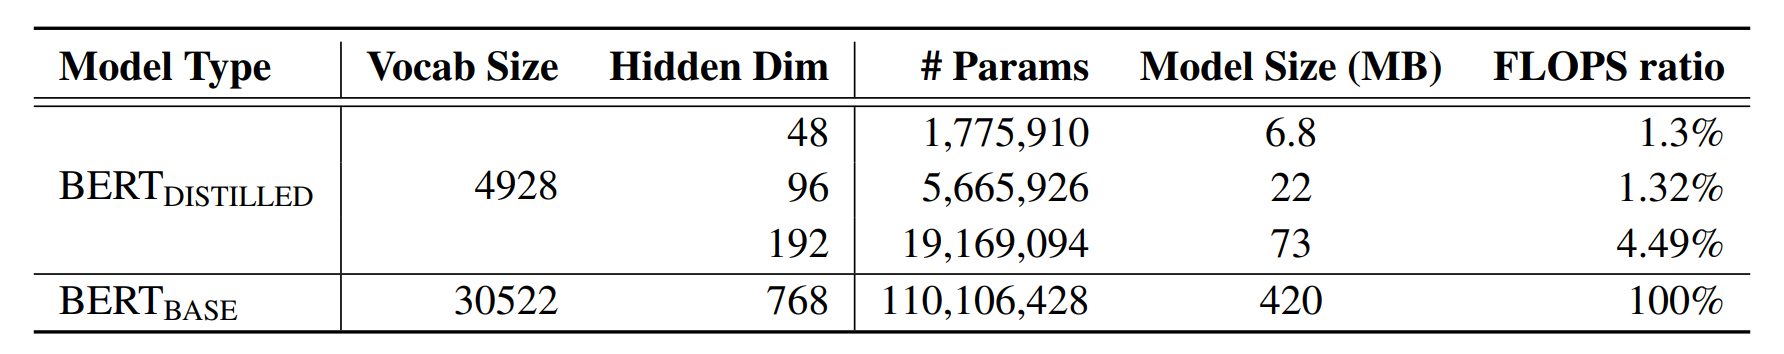
\includegraphics[width=0.9\linewidth]{images/power}
	\label{fig:seq2seq}
\end{figure}
\end{frame}

\begin{transitionframe}
	\begin{center}
		\Huge  ELMO
	\end{center}
\end{transitionframe}

\begin{frame}{Серия вопросов в зал}
Как работают разные эмбединги?

В чем, по вашему мнению, их главная проблема?
\end{frame}

\begin{frame}{Картиночка про решение проблемы}

\begin{figure}
	\centering
	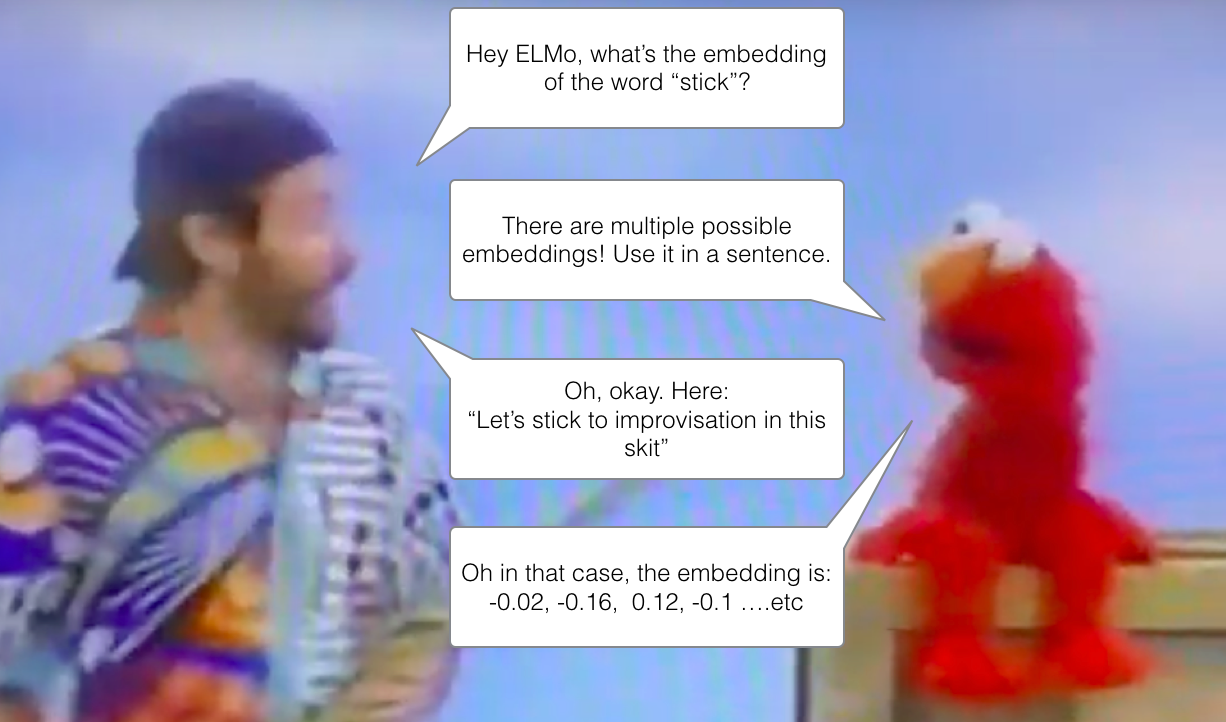
\includegraphics[width=0.9\linewidth]{images/elmo-embedding-robin-williams}
	\label{fig:seq2seq}
\end{figure}
\end{frame}

\begin{frame}{ELMO}
	
Захватываем контекст предложения через biderictional LSTM. Таким образом мы захватываем и контекст предложения (да, надо очень очень много данных, не обучайте это дома)



\begin{figure}
	\centering
	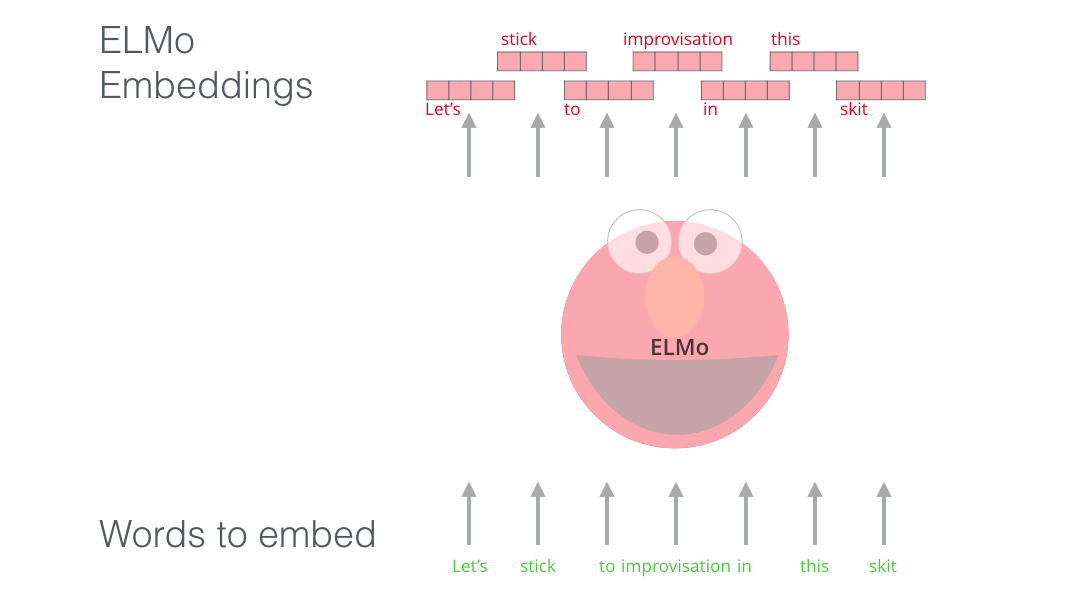
\includegraphics[width=0.7\linewidth]{images/elmo-word-embedding}
	\label{fig:seq2seq}
\end{figure}
\end{frame}


\begin{frame}{ELMO}
	Учится понимать язык ELMO следующим образом - оно берет большой дата сет и пытается предсказать следующее слово в предложении.	
	\begin{figure}
		\centering
		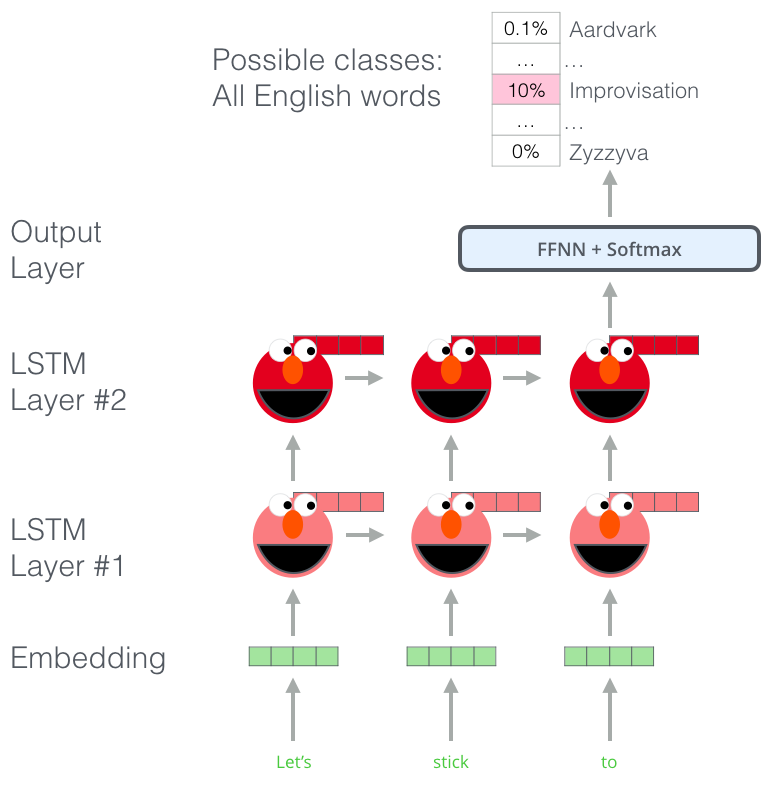
\includegraphics[width=0.4\linewidth]{images/Bert-language-modeling}
		\label{fig:seq2seq}
	\end{figure}
\end{frame}

\begin{frame}{ELMO}
	Применяем	
	\begin{figure}
		\centering
		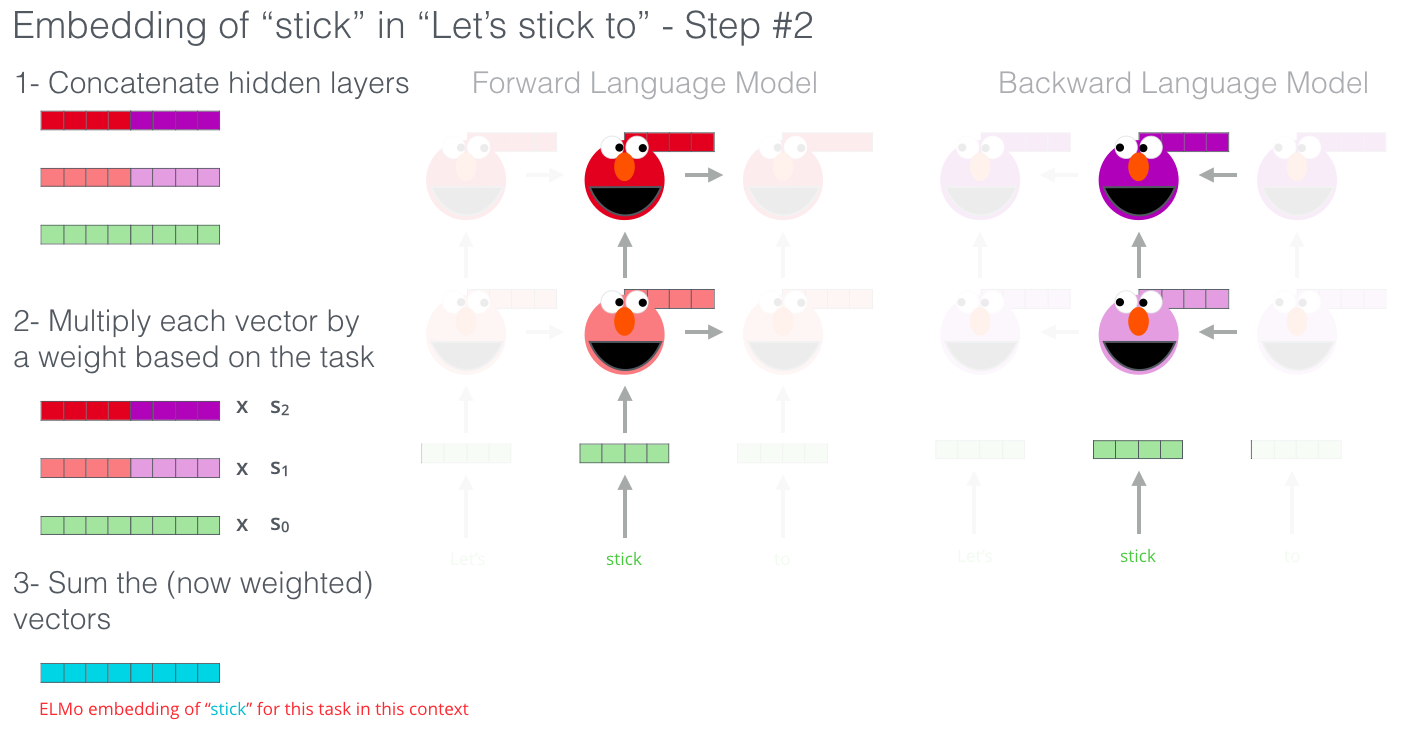
\includegraphics[width=0.75\linewidth]{images/elmo-embedding}
		\label{fig:seq2seq}
	\end{figure}
\end{frame}


\begin{frame}{ELMO}
	Применяем	
	\begin{figure}
		\centering
		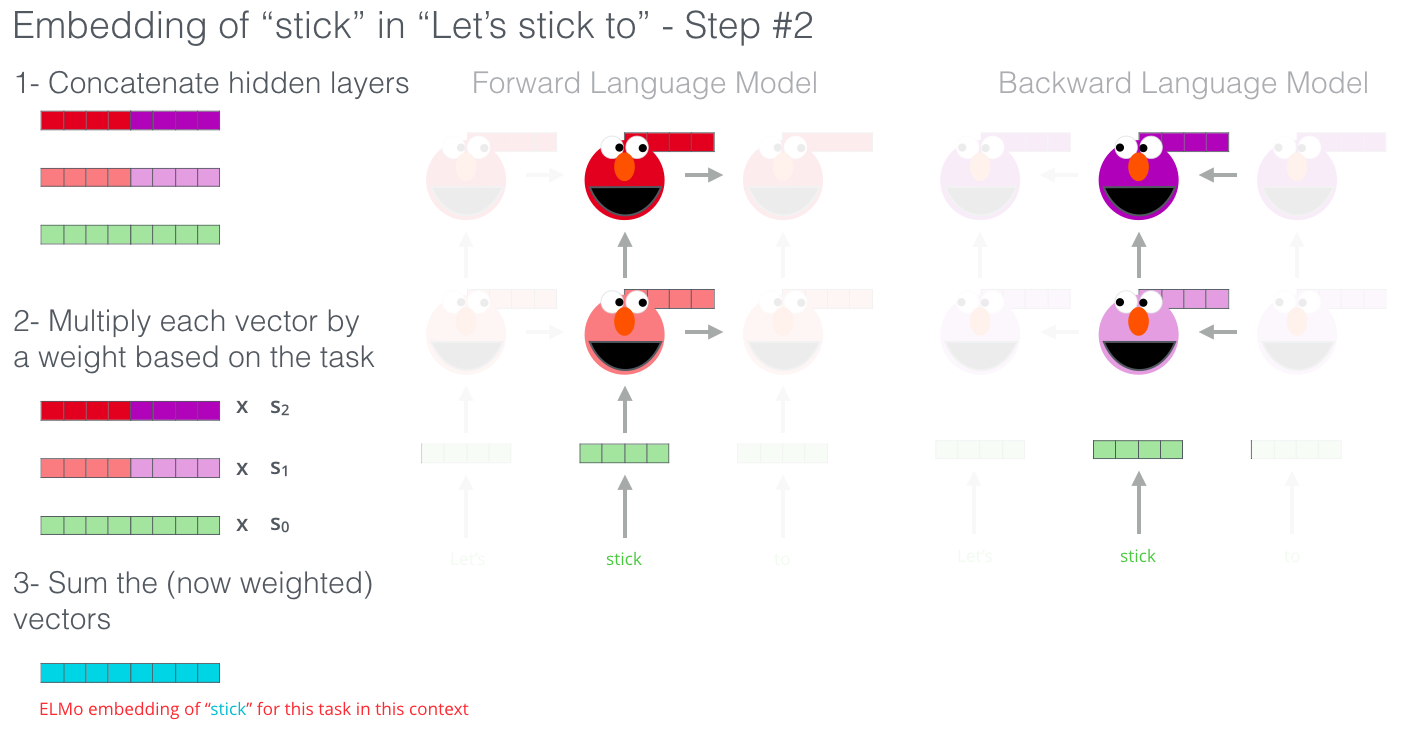
\includegraphics[width=0.75\linewidth]{images/elmo-embedding}
		\label{fig:seq2seq}
	\end{figure}
\end{frame}

\begin{frame}{Итого}
Почему это все стало круто и популярно?
\begin{enumerate}
	\item Идея с вниманием стала ключевой - таким образом мы можем тянуть информацию через всю последовательность
	\item Внимание можно параллелизовать, LSTM намного сложнее
	\item Придумали как сделать так, чтобы не размечать данные
	\item Купили много GPU
	\item  Посадили кучу инженеров, которые заставили это все учиться!
\end{enumerate}
Ну и маленькая мысль в конце - за курс мы разобрали кубики нейронных сетей и посмотрели какой лютый треш можно из этих кубиков делать. Современный моделист в нейронных сетях - скорее инженер, нежели аналитик
\end{frame}

\end{document}
